% !TeX spellcheck = cs_CZ
%---------------------------------------------------------------------------------------------------
% mai2ch01.tex
%---------------------------------------------------------------------------------------------------
\chapter{Vícerozměrná linearita aneb lineární algebra podruhé}\label{mai:IIchapI}
\minitoc
  V kapitole \ref{mai:IchapII} dílu \ref{part:MAI} jsme se seznámili s elegantní dámou lineární 
  algebrou. Pomocí jejích pravidel jsme nejen řešili soustavy lineárních rovnic, ale také počítali 
  s maticemi a vektory. Zatímco operace s maticemi, a koneckonců i řešení lineárních rovnic pomocí 
  matic bychom mohli chápat jako užitečnou ekvilibristiku s číselnými soubory, za počítáním s 
  vektory se zdálo být přece jen něco hlubšího a závažnějšího. Vázané vektory pro nás totiž byly 
  orientovanými úsečkami v trojrozměrném euklidovském prostoru, v němž bylo definováno měření délek 
  a úhlů. Volné vektory pak byly množinami stejně velkých a souhlasně rovnoběžných orientovaných 
  úseček. Jednalo se tedy o \emph{geometrické objekty}. Každý vektor byl určen svou velikostí a 
  směrem. Směr byl přitom zadán například pomocí úhlů mezi daným vektorem a vybranými směry, které 
  byly předem pevně zvoleny. Mohli jsme s vektory provádět základní algebraické operace, jimiž jsou 
  sčítání vektorů a násobení vektoru číslem, podle pravidel zavedených pro (v tomto případě 
  řádkové) matice. S vektory v trojrozměrném prostoru jsme mohli velmi pohodlně počítat jako s 
  trojicemi čísel. Na druhé straně jsme vektory vyjadřovali jako lineární kombinace jiných vektorů, 
  tvořících v prostoru všech vektorů \emph{bázi}. Koeficienty lineární kombinace, která 
  představovala zápis daného vektoru ve zvolené bázi, byly jeho \emph{složkami} v této bázi. Při 
  změně báze se změnily složky vektoru, vektor sám však nikoliv. Vektor je stále sám sebou, jen se 
  v různých bázích jinak tváří - projeví se jinou trojicí čísel. Protože se však při změně báze 
  změní složky vektoru přesně definovaným způsobem (vzpomeňte na transformační vztahy), dokážeme 
  jej vždy rozpoznat. Tuto vlastnost, \emph{invarianci vůči volbě báze}, mají všechny geometrické 
  objekty. A je to právě algebra, která nám umožňuje tyto objekty reprezentovat číselnými soubory a 
  také tak s nimi počítat. Jde-li navíc o objekty řídící se lineárními pravidly. jakými jsou 
  například distributivní zákony, je počítání s nimi, v rámci \emph{lineární algebry}, zvláště 
  jednoduché. Oceníme to zejména v prostorech vyšší dimenze, než je náš běžný euklidovský prostor. 
  Při počítání s vektory v trojrozměrném prostoru, kde umíme měřit délky a úhly a kde platí 
  trigonometrická pravidla, bychom se bez rutinních algebraických procedur ještě třeba obešli. Už 
  ale například ve čtyřrozměrném časoprostoru, v němž se odehrávají všechny přírodní jevy a v němž 
  je třeba formulovat fyzikální zákony, však pro měření délek a úhlů platí jiná pravidla, než jsou 
  obvyklá v běžném, tj. trojrozměrném euklidovském, prostoru. Například tam neplatí čtyřrozměrná 
  verze Pythagorovy věty. A někdy je příroda dokonce tak nepřívětivá, že nás nutí pracovat i s 
  prostory vícerozměrnými. Například jedna z velmi účinných teorií pro výklad chování elementárních 
  částic, teorie strum, je založena na geometrii prostoru jedenáctirozměrného. A v takových 
  dimenzích jsme už s jakkoli vynikající geometrickou představivostí v koncích. Tehdy se vděčně 
  obracíme k metodám algebry. V této kapitole, jak její název napovídá, půjde o algebru lineární
  
  \section{Prostory s vektory}
    V kapitole \ref{mai:IchapII} jsme pracovali s číselnými maticemi typu \(m/n\), tj. soubory 
    čísel uspořádaných v \(m\) řádcích a \(n\) sloupcích, a zavedli jsme pro ně operaci součtu a 
    násobení číslem. Zjistili jsme, že pro sčítání matic a násobení matice číslem platí určitá 
    pravidla. (Jejich souhrn je uveden v samém závěru odstavce \ref{mai:IchapIIsecIIIsubIII}. V 
    odstavci \ref{mai:IchapIIsecIV} jsme zase počítali s vektory. Ty měly jednou \emph{konkrétní 
    podobu} řádkových matic s pravidly pro jejich sčítání a násobení číslem, podruhé, v 
    trojrozměrném prostoru, naopak \emph{konkrétní podobu} orientovaných úseček, resp. množin, 
    které byly orientovanými úsečkami vytvořeny, generovány. Zavedli jsme tenkrát konkrétní způsob 
    sčítání vektorů a násobení vektoru číslem pomocí geometrických operací. Součet dvou vektorů 
    \(\vec{u}\) a \(\vec{v}\) znamenal, že jsme podle zcela určitého pravidla, pravidla 
    vektorového rovnoběžníka přiřadili uspořádané dvojici \([\vec{u},\vec{v}]\) třetí vektor 
    \(\vec{u} + \vec{v}\), násobek vektoru a čísla byl opět vektor \(\alpha\vec{u}\), který jsme 
    přiřadili dvojici \([\alpha,\vec{u}]\) tvořené číslem a vektorem. Uvedli jsem, že pravidla pro 
    tyto \emph{geometrické} operace jsou shodná s pravidly pro počítání s maticemi a lze je dokázat 
    i geometrickými postupy. Množinu volných vektorů generovaných orientovanými úsečkami spolu s 
    uvedenými dvěma operacemi jsme nazvali \textbf{vektorovým prostorem}. Šlo tedy o zcela odlišné 
    množiny základních objektů a zcela odlišným způsobem definované operace, pro které se však dala 
    dokázat tatáž pravidla. Nyní se podíváme na problém definice vektorového prostoru obecněji a 
    poněkud \uv{opačně}. Budeme pracovat s \emph{nosnou množinou} \(V\), a přitom nebude podstatné, 
    jak konkrétně vypadají její prvky. Ani je nebudeme označovat šipkami (u šipek ze zvyku 
    zůstaneme pouze v případě orientovaných úseček v \(\mathbb{R}^1\), \(\mathbb{R}^2\) a 
    \(\mathbb{R}^3\), nebo vektorů s fyzikálním významem). Dále přibereme do hry množinu všech 
    komplexních čísel \(\mathbb{C}\), popřípadě jen množinu všech reálných čísel \(\mathbb{R}\) a 
    definujeme dvě operace (\emph{zobrazení}):
    \begin{equation}\label{mai:eq046}
      V \times V \ni [a,b] \longrightarrow c\in V,\qquad 
      \mathbb{C}\times V\ni[\alpha,a] \longrightarrow d\in V.
    \end{equation}
    Prvek \(c\) nazýváme \emph{součet} prvků \(a\) a \(b\) a značíme jej \(c = a + b\) prvek \(d\) 
    je \(\alpha\)-\emph{násobek} prvku \(a\) a značíme \(d = \alpha a\). Zobrazení uvedená ve 
    vztazích (\ref{mai:eq046}) však nebudou moci být úplně libovolná. Budeme požadovat, aby měla 
    určité vlastnosti, konkrétně ty, které jsou uvedeny pro matice na konci odstavce 
    \ref{mai:IchapIIsecIIIsubIII}. Teprve pak řekneme, že množina \(V\) spolu s operacemi 
    (\ref{mai:eq046}) splňujícími potřebné požadavky je vektorovým prostorem. Vidíme, že takto naše 
    uvažování výrazně posuneme na abstraktní úroveň. Bude lhostejné, co jsou prvky nosné množiny, 
    bude nepodstatné, jak konkrétně jsou definovány operace sčítání prvků a násobení prvku číslem. 
    Důležité bude jen to, aby abstraktní operace s abstraktními prvky splňovaly konkrétní pravidla. 
    Než však k definici vektorového prostoru přistoupíme, všimneme si ještě některých jiných 
    struktur s jednou nebo dvěma operacemi, které samy do oblasti lineární algebry nepatří, ale 
    mohou být užitečné pro definici vektorového prostoru, popřípadě mají významné fyzikální 
    aplikace.
      
      \subsection{Algebraické struktury s jednou operací, hlavně grupy}
        Při zavádění operací s vektory jsme zcela automaticky využívali toho, že umíme počítat s 
        reálnými, popřípadě i s komplexními čísly. Skutečnost, že čísla umíme sčítat, násobit a 
        provádět s nimi řadu dalších operací, považujeme za tak přirozenou a samozřejmou, že nad ní 
        vůbec nepřemýšlíme. Již samotné operace sčítání a násobení vytvářejí na množině čísel velmi 
        bohatou \textbf{algebraickou strukturu}. Tento pojem si nyní přiblížíme. 
        
        Algebraickou strukturu s jednou operací získáme, vezmeme-li v úvahu první ze zobrazení 
        (\ref{mai:eq046}), nosnou množinu označíme tentokrát podle zvyku \(G\):
        \begin{equation}\label{mai:eq047}
          G \times G \ni [a,b] \longrightarrow a + b \in G, \qquad \text{nebo} \qquad
          G \times G \ni [a,b] \longrightarrow a \cdot b \in G.
        \end{equation}
        Pokud použijeme první možnosti označení této operace, hovoříme o operaci \emph{sčítání} a 
        \emph{aditivní} struktuře, v případě druhé možnosti o operaci \emph{násobení} a 
        \emph{multiplikativní} struktuře. Toto terminologické rozlišení nemá obecně žádný hlubší 
        význam. Je spíše otázkou zvyklosti a souvisí především s algebraickou strukturou číselných 
        množin, kterou běžně používáme, aniž o ní přemýšlíme (čísla sčítá a násobí školák, 
        obchodník i účetní a o nějaké abstraktní struktuře nic netuší).
        
        Zobrazení (\ref{mai:eq047}) samo o sobě, aniž na ně klademe další požadavky (podstatné je 
        pouze to, že dvěma prvkům nosné množiny přiřadí prvek \emph{téže množiny}), definuje 
        nejjednodušší algebraickou strukturu s jednou operací, zvanou \textbf{grupoid}. Grupoid 
        není pro fyzikální aplikace příliš užitečný, ale je základem pro konstrukci zajímavějších a 
        užitečnějších struktur. Přidáme-li k definici grupoidu požadavek \emph{asociativity} 
        zobrazení \(G \times G \ni [a, b] \longrightarrow a + b \in G\) (nebo \(G \times G \ni [a, 
        b] \longrightarrow a \cdot b \in G\))
        \begin{equation}\label{mai:eq048}
          (a+b) + c = a + (b + c),\qquad \text{nebo}\qquad (a\cdot b) \cdot c = a \cdot (b \cdot c)
        \end{equation}
        pro libovolné prvky \(a, b, c \in G\), stane se množina \(G\) spolu s operací „\(+\)“, nebo 
        „-“ \textbf{pologrupou}. I pologrupa je z hlediska fyzikálních aplikací poněkud chudá, 
        další požadavek na zobrazení (\ref{mai:eq047}) z ní však již učiní strukturu v matematice i 
        fyzice nepostradatelnou, grupu. Pologrupa, ve které existuje prvek \(0_G\in G\) a současně 
        ke každému prvku \(a \in G\) existuje prvek \((-a) \in G\) tak, že platí
        \begin{equation}\label{mai:eq049}
          a + 0_G = 0_G + a = a,\qquad a + (-a) = (-a) + a = 0_G,
        \end{equation}
        se nazývá \textbf{aditivní grupou}. Prvek \(0_G\) je univerzální pro celou grupu (žádný 
        jiný s touto vlastností v grupě \(G\) není) a nazývá se \emph{neutrální prvek grupy} neboli 
        \textbf{nula}, prvek \((-a)\) je \textbf{opačný} k prvku \(a\). Pro dané \(a\) je určen 
        jednoznačně. V případě operace násobení mají vlastnosti \ref{mai:eq049} tvar
        \begin{equation}\label{mai:eq050}
          a \cdot e_G = e_G \cdot a = a,\qquad a \cdot a^{-1} = a^{-1} \cdot a = e_G,
        \end{equation}
        a \(G\) se nazývá \textbf{multiplikativní grupou}. Prvek \(e_G\) je opět univerzální pro 
        celou grupu a nazývá se \textbf{neutrální} prvek grupy, neboli \emph{jednička}, prvek 
        \(a^{-1}\) je \textbf{inverzní} k prvku \(a\).
        
        Každá operace \ref{mai:eq047} v množině \(G\), která splňuje vztahy asociativity 
        \ref{mai:eq048} a vztahy specifikující nulu a opačný prvek, nebo jedničku a inverzní prvek 
        typu \ref{mai:eq049}, nebo \ref{mai:eq050}, představuje \emph{grupovou operaci} bez ohledu 
        na to, podobá-li se spíše sčítání, nebo spíše násobení, či dokonce něčemu jinému, například 
        skládání zobrazení. Má-li grupa konečný počet prvků, nazývá se tento počet jejím 
        \emph{řádem}.

        %---------------------------------------------------------------
        % !TeX spellcheck = cs_CZ
\wikitextrule
\begin{example}\label{mai:exam046}
  \textbf{Kolik nul má (aditivní) grupa?}\newline\small
  Jak dokážeme, že má grupa právě jednu nulu? Co když předchozímu tvrzení nebudeme věřit? Můžeme se 
  o jeho pravdivosti přesvědčit? Ten, kdo mu nevěří, si může třeba představit, že grupa má nuly 
  dvě. Označme je \(0_G\) a \(\overline{0}_G\). Vztah \ref{mai:eq049} platí pro libovolný prvek 
  grupy, proto \(0_G + \overline{0}_G = 0_G\) (to jsme brali \(a = 0_G\) a \(\overline{0}_G\) 
  považovali za nulu) a současně \(0_G + \overline{0}_G = \overline{0}_G\) (nyní zase byl prvek 
  \(0_G\) v roli nuly a \(a = \overline{0}_G\)). Je vidět, že \(0_G = \overline{0}_G\). Nula je 
  tedy skutečně jen jedna. Podobnou úvahu můžeme provést pro jedničku multiplikativní grupy. Platí 
  tedy tvrzení:
  
  \noindent
  \adjustbox{}{Neutrální prvek grupy je určen jednoznačně.}

  
  Stejně tak bychom mohli mít pochybnosti o tom, že opačný prvek k danému \(a\in G\) je jen jeden. 
  Předpokládejme, že \(b\) a \(c\) jsou dva opačné prvky k \(a\). Platí \(a + b = 0_G\). Přičteme k 
  této rovnosti \(c\) zleva, tj. \(c + a + b = c\). Protože však \(c + a = 0_G\), dostáváme \(b=c\) 
  a tedy:
 
  \noindent
  \adjustbox{}{Opačný (resp. inverzní) prvek k libovolně zvolenému prvku grupy je určen 
  jednoznačně.}
  \normalsize
\end{example}
        %---------------------------------------------------------------
        
        V úvodu odstavce jsme se zmínili o tom, že množiny reálných a komplexních čísel získají 
        zavedením běžných operací sčítání a násobení jistou algebraickou strukturu. Všimněme si 
        jich nyní podrobněji. 
        
        %---------------------------------------------------------------
        % !TeX spellcheck = cs_CZ
\wikitextrule
\begin{example}\label{mai:exam047}
  \textbf{Algebraická struktura a kupecké počty}\newline\small
    Uvažujme o množině reálných čísel \(G = \mathbb{R}\) tak, jako bychom je uměli jen 
    sčítat. Násobení si zatím nevšímejme. Sčítání reálných čísel je zobrazení typu prvního 
    vztahu v \ref{mai:eq047}, které bezpochyby splňuje požadavky \ref{mai:eq048} a 
    \ref{mai:eq049}. Neutrálním prvkem \(0_\mathbb{R}\) je \uv{obyčejná} nula, opačným prvkem k 
    číslu \(a\) je \(-a\), položené na reálné ose symetricky k \(a\) vzhledem k nule. Množina 
    reálných čísel s operací sčítání je tedy aditivní grupou. Pro operaci sčítání dokonce platí 
    něco navíc - komutativní zákon
    \begin{equation}\label{mai:eq051}
      a + b = b + a \qquad\text{pro libovolné}\qquad a,b\in\mathbb{R}.
    \end{equation} 
    Grupu s komutativním zákonem nazýváme grupou \emph{komutativní} nebo také \textbf{abelovskou}.
    
      \adjustbox{}{Množina reálných čísel s operací sčítání je komutativní grupou.}
    
    Nyní se místo na sčítání zaměřme na násobení reálných čísel a znovu posuďme vlastnosti grupy. 
    Násobení reálných čísel je zobrazením typu druhého vztahu v \ref{mai:eq047} a splňuje požadavek 
    asociativnosti \ref{mai:eq048}. Dále je zřejmé, že číslo \(e_\mathbb{R}\) (\uv{obyčejná} 
    jednička) vyhovuje prvnímu požadavku ve vztazích \ref{mai:eq050}. Potíž je s požadavkem druhým. 
    Inverzní prvek najdeme jen k nenulovým číslům. Nula inverzní prvek nemá. Tato zdánlivá drobnost 
    je příčinou toho, že \textbf{množina reálných čísel s operací násobení není grupou}.
  \normalsize
\end{example}
        %---------------------------------------------------------------
        
        %---------------------------------------------------------------
        % !TeX spellcheck = cs_CZ
\wikitextrule
\begin{example}\label{mai:exam048}
  \textbf{Algebraická struktura na množině komplexních čísel}\newline\small
    Množina \(\cmplxset\) komplexních čísel je kartézským součinem reálných os, \(\cmplxset = 
    \mathbb{R} \times \mathbb{R}\), tedy množinou uspořádaných dvojic \([a, b]\) čísel reálných. 
    Značíme \(z = [a, b]\). Reálné číslo \(a = \operatorname{Re}(z)\) je \emph{reálnou} částí 
    komplexního čísla \(z\) a reálné číslo \(b = \operatorname{Im}(z)\) částí \emph{imaginární}. 
    Operace sčítání a násobení komplexních čísel jsou definovány takto:
    \begin{align*}
      \cmplxset\times\cmplxset\ni\left[[a_1, b_1],[a_2, b_2]\right] &\longrightarrow
        [a_1, b_1] + [a_2, b_2] = [a_1 + a_2, b_1 + b_2]\in\cmplxset,                   \\
      \cmplxset\times\cmplxset\ni\left[[a_1, b_1],[a_2, b_2]\right] &\longrightarrow
        [a_1, b_1] \cdot [a_2, b_2] = 
        [a_1 \cdot a_2 - b_1 \cdot b_2, a_1 \cdot b_2 + a_2 \cdot b_1]\in\cmplxset.
    \end{align*}
    
    \adjustbox{}{Množina komplexních čísel s operací součtu je komutativní grupou.}
    
    Jejím neutrálním prvkem je číslo \(0_\cmplxset = [0,0]\), opačným prvkem k číslu \(z = [a, b]\) 
    je \(-z = [-a, - b]\). Při operaci násobení je neutrálním prvkem číslo [1,0], prvkem inverzním 
    k číslu \(z = [a, b] \neq 0_\cmplxset\) je
    \begin{equation*}
      z^{-1} = \left[\dfrac{a}{a^2 + b^2}, \dfrac{-b}{a^2 + b^2}\right].
    \end{equation*}
    
    K číslu \(0_\cmplxset = [0,0]\) však inverzní prvek opět neexistuje. Množina komplexních čísel 
    \textbf{není grupou vzhledem k násobení}.
  \normalsize
\end{example}
        %---------------------------------------------------------------
        
        O podmnožině \(H \subset C\) grupy \(G\) s operací sčítání nebo násobení zúženou na \(H\), 
        která je sama grupou, hovoříme jako o \textbf{podgrupě} grupy \(G\). Například množina 
        reálných čísel zapsaných ve tvaru \(z = [a, 0]\) se sčítáním je podgrupou množiny 
        komplexních čísel. Koho grupy nebaví a chce se rychle prokousat k vektorovým prostorům, 
        které jsou koneckonců hlavní náplní našeho příběhu o lineární algebře, může zbytek tohoto 
        odstavce přeskočit. Ale byla by to škoda, grupy jsou opravdu zajímavé.

        %---------------------------------------------------------------
        % !TeX spellcheck = cs_CZ
\wikitextrule
\begin{example}\label{mai:exam050}
  \textbf{Struktura aditivní grupy na podmnožinách reálné osy}\newline\small

  \normalsize
\end{example}
        %---------------------------------------------------------------
        
        %---------------------------------------------------------------
        % !TeX spellcheck = cs_CZ
\wikitextrule
\begin{example}\label{mai:exam050}
  \textbf{Grupy některých číselných objektů}\newline\small

  \normalsize
\end{example}
        %---------------------------------------------------------------

        %---------------------------------------------------------------
        % !TeX spellcheck = cs_CZ
\wikitextrule
\begin{example}\label{mai:exam051}
  \textbf{Grupy nemusí být tvořeny jen čísly}\newline\small
  {\centering
    \captionsetup{type=figure}
    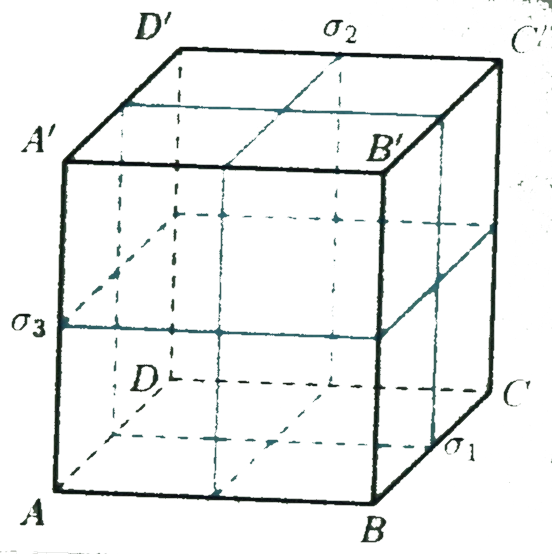
\includegraphics[width=0.4\linewidth]{mai_fig037.png}
    \captionof{figure}{Zadáni přímky. \cite[s.~6]{Musilova2012MA2}
    \label{mai:fig000}}
    \par}
  \normalsize
\end{example}
        %---------------------------------------------------------------
        
      \subsection{Algebraické struktury se dvěma operacemi, hlavně pole}
      
      \subsection{Co je to vektorový prostor?}
  
  \section{Lineární zobrazení vektorových prostorů}

%---------------------------------------------------------------------------------------------------
\printbibliography[title={Seznam literatury}, heading=subbibliography]
\addcontentsline{toc}{section}{Seznam literatury}